
\appendix

\section{Effect of Control Strength}

\begin{figure}[ht]
    \centering
    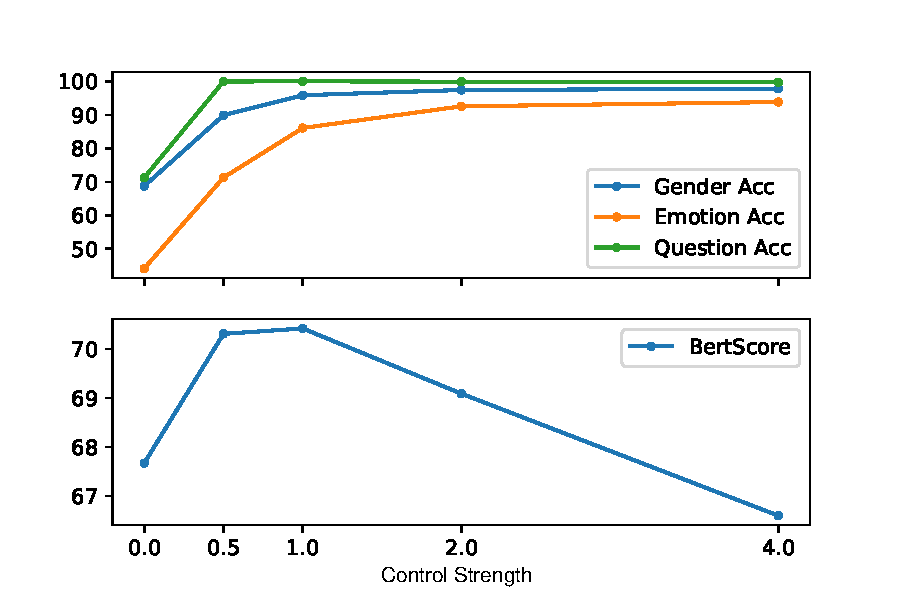
\includegraphics[width=1.0\columnwidth]{figures/parameter_tune.pdf}
    \caption{Effect of control strength on controllability and generation quality}
    \label{fig:parameter_tune}
\end{figure}

We show the effect of control strength $\alpha$ (\eqnref{eqn:dasc_logits}) on DASC's controllability and generation quality in Figure \ref{fig:parameter_tune}. From the trend shown in this figure, we can see that for \textit{Question} which is easy to control, we can already achieve perfect control with a low $\alpha$, while harder attributes like \textit{Emotion} would require a higher $\alpha$ to get a high success rate. Therefore, we may further hypothesize that a better balancing of the control accuracy of each attribute and the generation quality can be achieved by setting different control strengths for each aspect, like higher $\alpha$ for Emotion and lower $\alpha$ for Question. Careful tuning of the parameters or specific searching algorithms \citep{gu2022distributional} may serve the goal, and we leave this for future work.\footnote{In practice, we further multiply $\alpha$ by the number of attributes $K$ to adapt to the variable attribute numbers, which is not counted in \eqnref{eqn:dasc_logits} and Figure \ref{fig:parameter_tune} for clarity.}

\section{Experiment Details}

For all experiment methods, they use \texttt{bart-base}\footnote{\url{https://huggingface.co/facebook/bart-base}} as the base model. All models are fine-tuned on the dataset for 6 epochs. When conducting multi-aspect control for Director and DASC under weighted-decoding paradigm (\eqnref{eqn:multi_wd_logits}), we set the variables for the desired attribute as 1, and other variables as $\phi$. The decoding method is top-$p$ sampling with $p=0.5$. DASC uses control weight $\alpha=1$ and classifier loss weight $\beta=0.1$, similar as the previous experiments. All experiments of the paper are conducted on a Linux server, and each experiment is run on a single NVIDIA A100 GPU. To avoid overfitting, we select the checkpoint with the best BertScore on dev set for final testing. We fix the random seed in experiment and report the results coming from a single run. Below we provide the specific details for the experiments on ESConv.

For experiments on ESConv \citep{liu2021towards}, we use the latest released version\footnote{\url{https://github.com/thu-coai/Emotional-Support-Conversation}}, which has 1,300 conversations, and we split them into 1,100/100/100 train/dev/test set, which contains 15,605/1,403/1,369 utterances each. In human evaluation, we further sample 15 utterances for each of the 7 emotional support strategies defined in the dataset (except the vague \textit{Other} class), and get 105 utterances in total. The meaning of \textbf{Sensibleness}$_{(1-4)}$ is similar to the experiment in the previous dataset: if the response is fluent, coherent with the context, and accords with commonsense. By \textbf{Usefulness}$_{(1-4)}$, we consider if the response dives deep in the problem faced by the support seeker, is comforting, contains useful suggestions or encourages in-depth further discussions. 

\section{Experiments with Description Control}
\label{sec:desc_control}

Dense persona descriptions are another common form of control signal in dialog generation \citep{zhang2018personalizing}, and we can also convert the sparse attributes into descriptive texts to be compatible with these methods. Therefore, we now supplement new experiment results with two representative methods that leverages persona descriptions for control.

\paragraph{BoB} \citep{song2021bob} disentangles the task of persona consistency learning and response generation, and leverages non-dialogue NLI datasets to help boost the performance of consistency learning and finally improves personalized generation. 

To apply BoB on the dataset we've experimented with, we convert the discrete attribute annotations into textual descriptions with rules. For example, the male/female gender will be converted to "I'm a girl/boy.", a question will have the description "I want to ask a question". And for emotion, we fill them in the template "I feel \{emotion\}." We concatenate these 3 description texts as the persona text to be used by BoB. As is suggested in the official GitHub repository, we leverage the Chinese NLI dataset CMNLI \citep{xu-etal-2020-clue} as the auxiliary inference datasets.

\paragraph{ChatGPT} \citep{openai2022:chatgpt} is a representative Large-Language-Model (LLM) that can follow human instruction and give responses. Therefore, we can encode the attribute values into the ChatGPT system message to achieve control on them. We use the template:

\begin{quote}
    A dialog history is given below. Please act as the \{current speaker\} and respond to the next sentence with a \{dialog act\} in the voice of \{gender and emotion\}.
\end{quote}

Then we use dialog history as the user message, and let ChatGPT (gpt-3.5-turbo) give a following sentence. We use temperature=0 and stop=``\textbackslash n'', that is, greedy search for one line of text similar to the setting of the original dataset. 


\begin{table}[h]
    \small
    \centering
    \begin{tabular}{cccccc}
    \hline
             & BScore         & Dist-2         & Acc$_G$         & Acc$_E$         & Acc$_Q$          \\ \hline
    Baseline & 68.18          & 19.25          & 68.49          & 46.31          & 69.61           \\
    CTRL     & \textbf{71.09} & 18.91          & 85.32          & 77.49          & \textbf{100.00} \\
    DASC     & 70.42          & 21.94          & \textbf{95.85} & \textbf{86.07} & \textbf{100.00} \\ \hline
    BoB      & 65.47          & 23.44          & 74.59          & 64.76          & 98.51           \\
    ChatGPT  & 66.21          & \textbf{30.98} & 69.49          & 56.88          & 98.22           \\ \hline
    \end{tabular}
    \caption{Automatic evaluation on the DuLemon test set with persona description-based controlling methods.}
    \label{tab:desc_control}
\end{table}

\begin{table}[h]
    \small
    \centering
    \begin{tabular}{ccc}
    \hline
            & Dist-2         & Acc$_E$         \\ \hline
    CTRL    & 21.07          & 43.38          \\
    DASC    & 26.71          & \textbf{65.38} \\ \hline
    BoB     & 24.25          & 30.13          \\
    ChatGPT & \textbf{37.02} & 30.00          \\ \hline
    \end{tabular}
    \caption{Automatic evaluation on the DuLemon robustness test with persona description-based controlling methods.}
    \label{tab:desc_control_robust}
\end{table}

Firstly, we can see that ChatGPT can generate highly diverse texts (with dist-2 on test set similar as the human ground truth, 30.98 VS 30.63). However, ChatGPT cannot achieve comparable controllability with finetuned methods like CTRL and DASC, especially on attributes whose manifestation cannot be easily described in the prompt (e.g. Gender and Emotion). 

Moreover, we can see that BoB also shows strong controllability compared to baseline and zero-shot ChatGPT. It also has higher generation diversity than other methods except ChatGPT, potentially due to the introduction of the auxiliary inference dataset. However, its controllability is relatively worse than DASC. Its generation quality is also poor, both reflected in the low BertScore and our manual check, where we find many influent cases like ``Yes. After all, I'm a lawyer, otherwise it would be hard to find a body.''. BoB also shows less sensitivity to the change of control signals, as is shown in the lower dist-2 and emotion accuracy in the robustness test. 

To conclude, we believe it is possible for description-based controllable generation methods like ChatGPT and BoB to perform better in the control of discrete attributes, but it would require significant efforts on prompt engineering (e.g. describe in more detail for ChatGPT, or make the description more similar to the auxiliary inference dataset for BoB). However, when we have relatively sufficient labeled data the discrete control attributes, DASC on `small' LMs will certainly be a simple and competitive choice.

\section{Examples and Visualizations}

In this section, we provide supplementary examples and figure visualizations. 

\begin{figure}[ht]
    \centering
    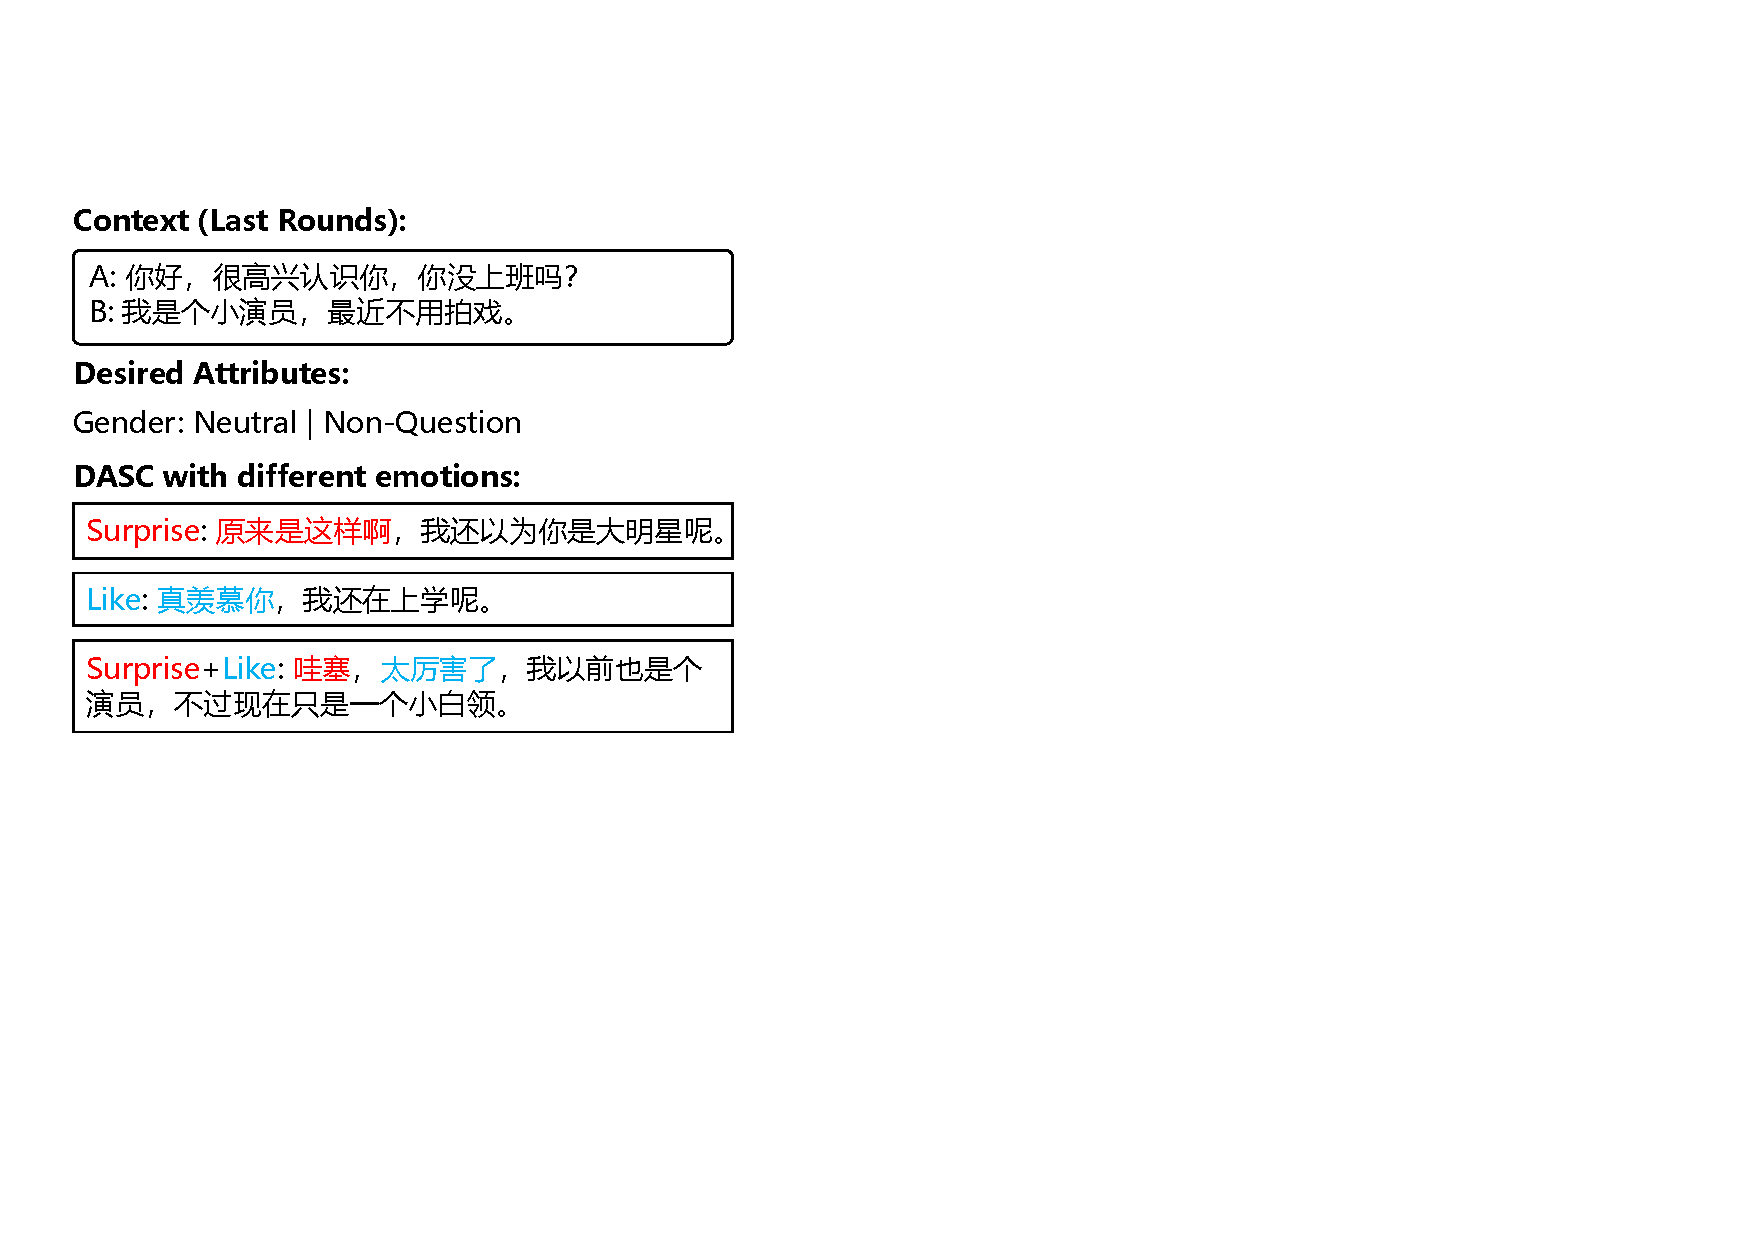
\includegraphics[width=1.0\columnwidth]{figures/compose_example1_zh.pdf}
    \caption{Original Chinese text for Figure \ref{fig:compose_example1_en}}
    \label{fig:compose_example1_zh}
\end{figure}

\begin{figure}[ht]
    \centering
    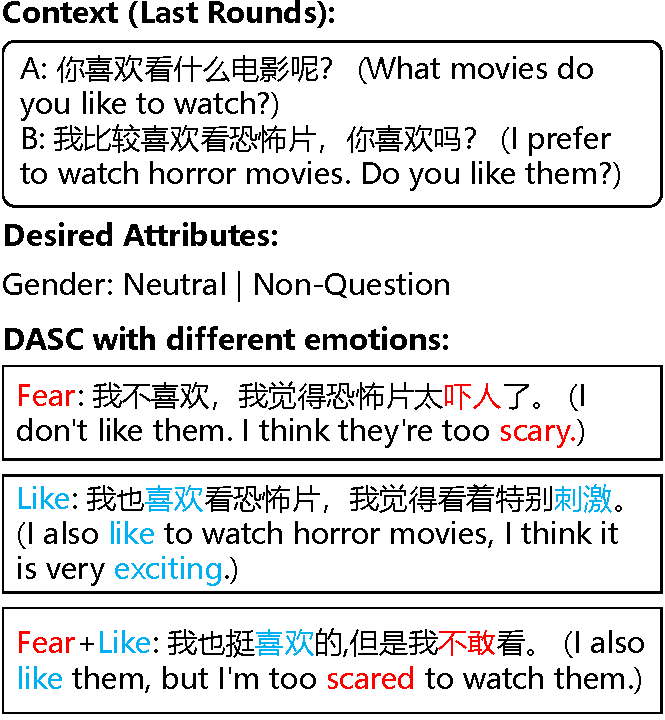
\includegraphics[width=1.0\columnwidth]{figures/compose_example2.pdf}
    \caption{Example of DASC composing \textit{Like} and \textit{Fear} 
emotion in the generated response.}
    \label{fig:compose_example2}
\end{figure}

Figure \ref{fig:compose_example1_zh} shows the original Chinese text for the emotion composition example in Figure \ref{fig:compose_example1_en}, and we provide another example in Figure \ref{fig:compose_example2}, which shows that DASC can even compose a positive emotion \textit{Like} and a negative emotion \textit{Fear} in the same response to express complex meanings. 

\begin{figure}[ht]
    \centering
    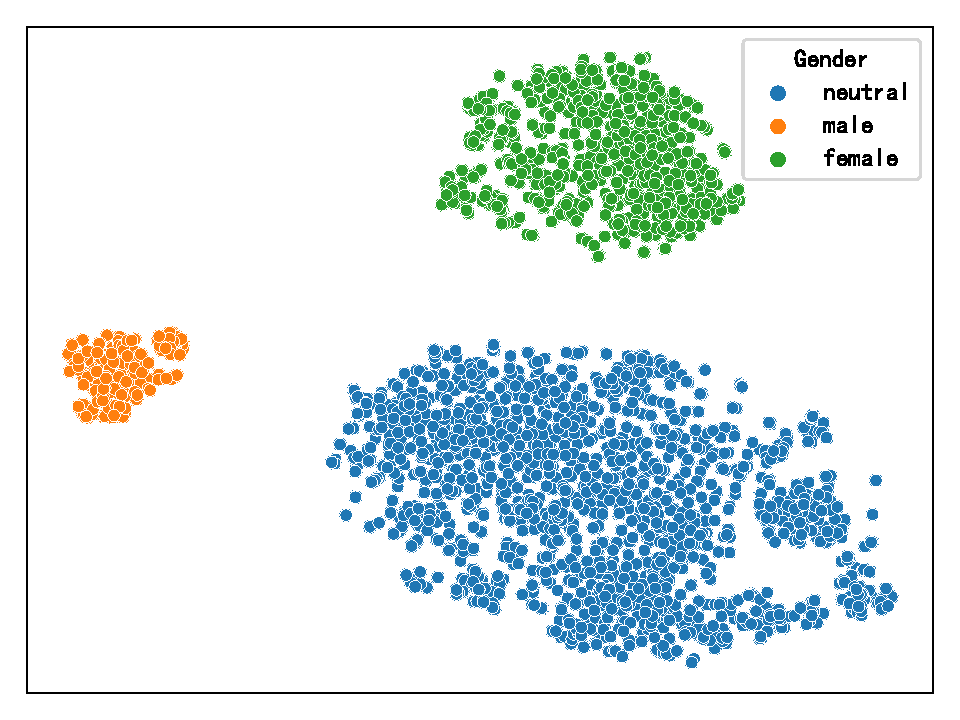
\includegraphics[width=1.0\columnwidth]{figures/gender_context_emb.pdf}
    \caption{Visualization of attribute context embedding of responses with different gender styles.}
    \label{fig:gender_context_emb}
\end{figure}

\begin{figure}[ht]
    \centering
    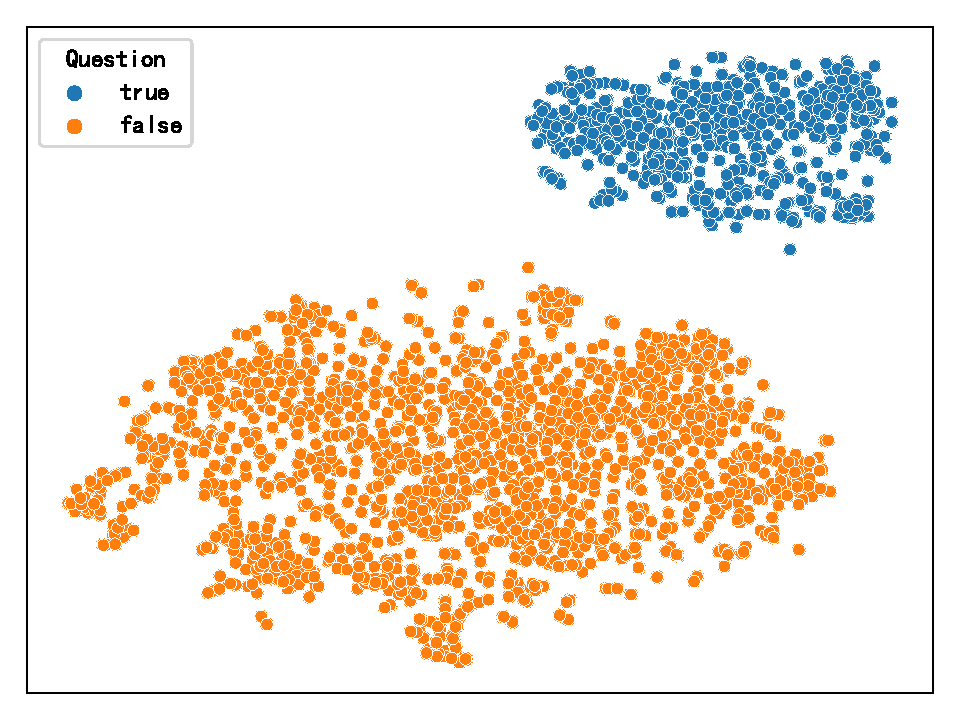
\includegraphics[width=1.0\columnwidth]{figures/question_context_emb.pdf}
    \caption{Visualization of attribute context embedding of responses with different question acts.}
    \label{fig:question_context_emb}
\end{figure}

We provide the t-SNE visualizations of attribute context embeddings of sentences with different \textit{Gender Style} and \textit{Question Act} in Figure \ref{fig:gender_context_emb} and Figure \ref{fig:question_context_emb}. We find similar results as we've seen for emotion, that the embeddings from different attributes are clearly separated.

\begin{figure}[htbp]
    \centering
    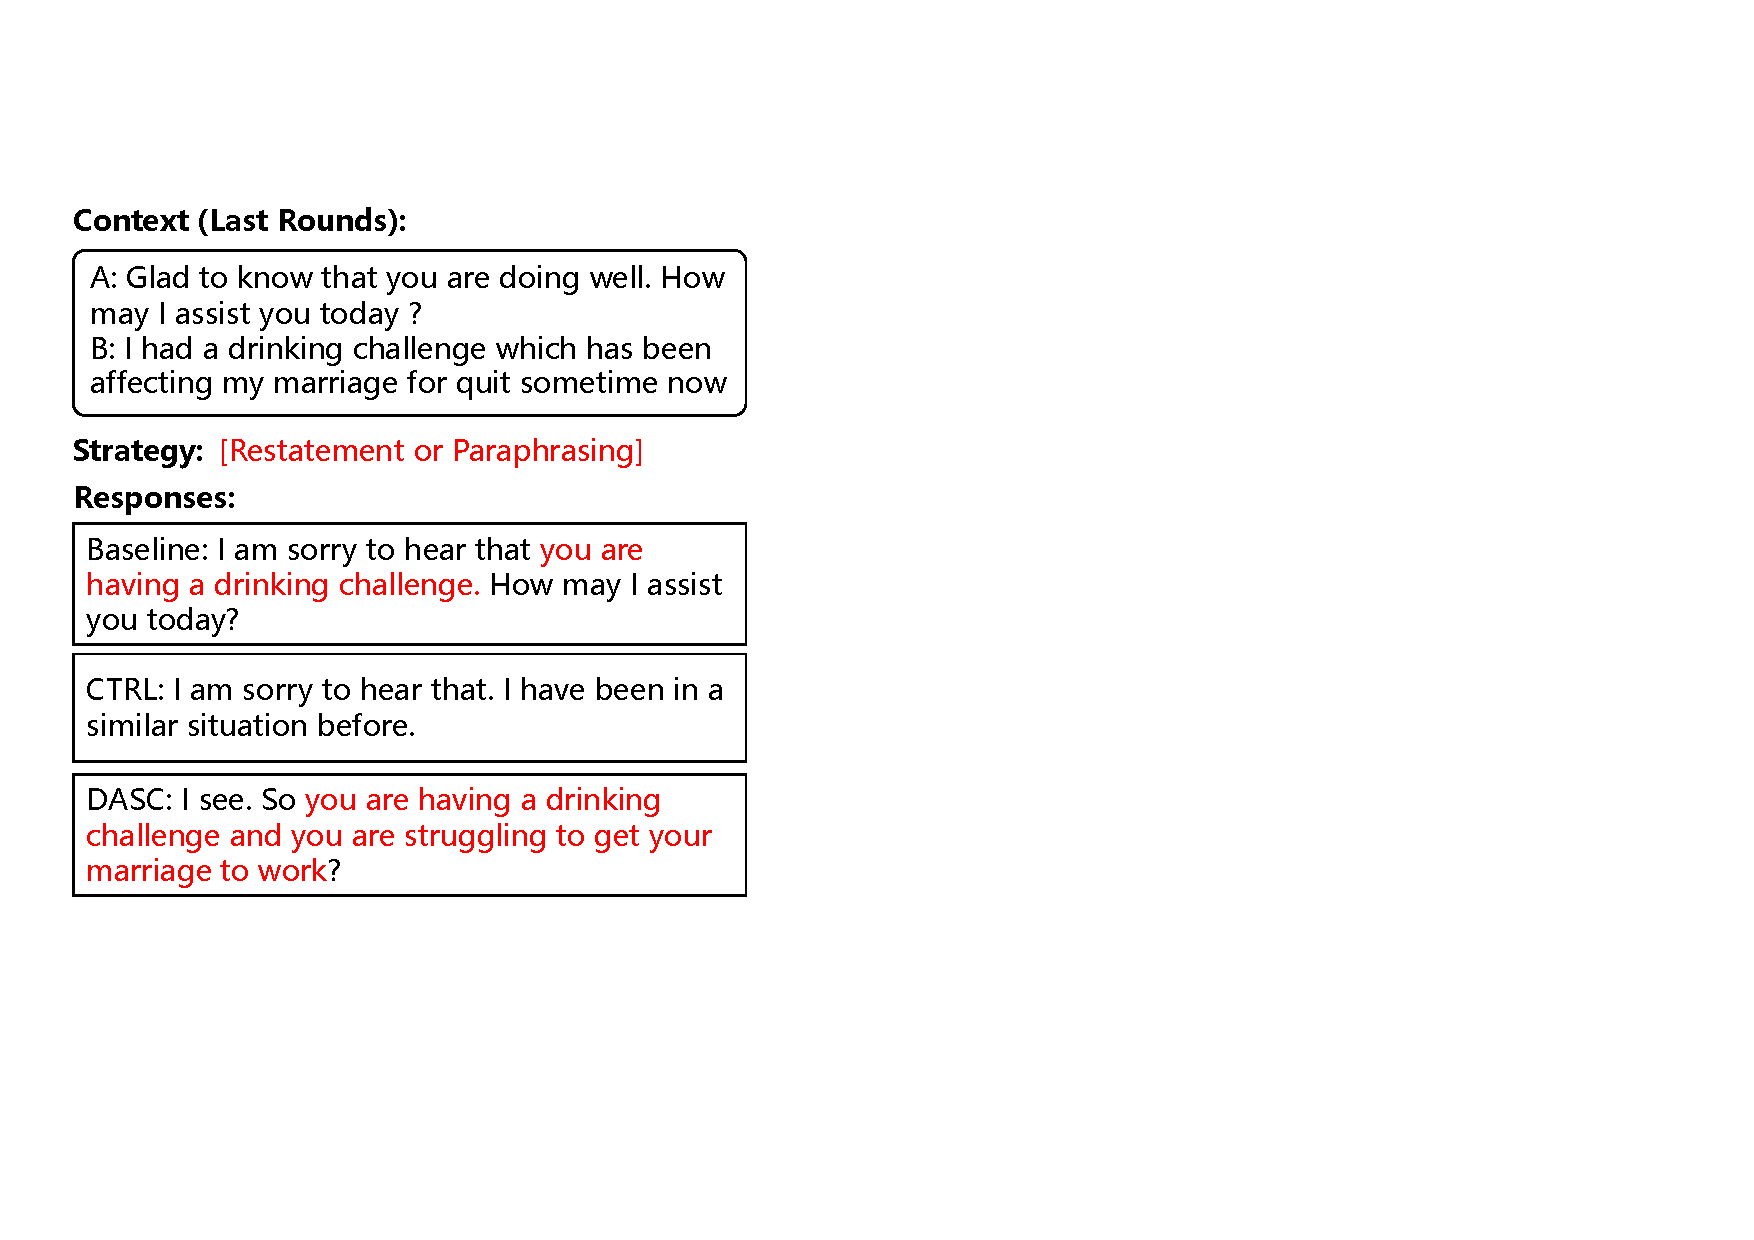
\includegraphics[width=1.0\columnwidth]{figures/esconv_example1.pdf}
    \caption{System generations in one example of ESConv, with the ``Restatement or Paraphrasing'' strategy.}
    \label{fig:esconv_example1}
\end{figure}

\begin{figure}[htbp]
    \centering
    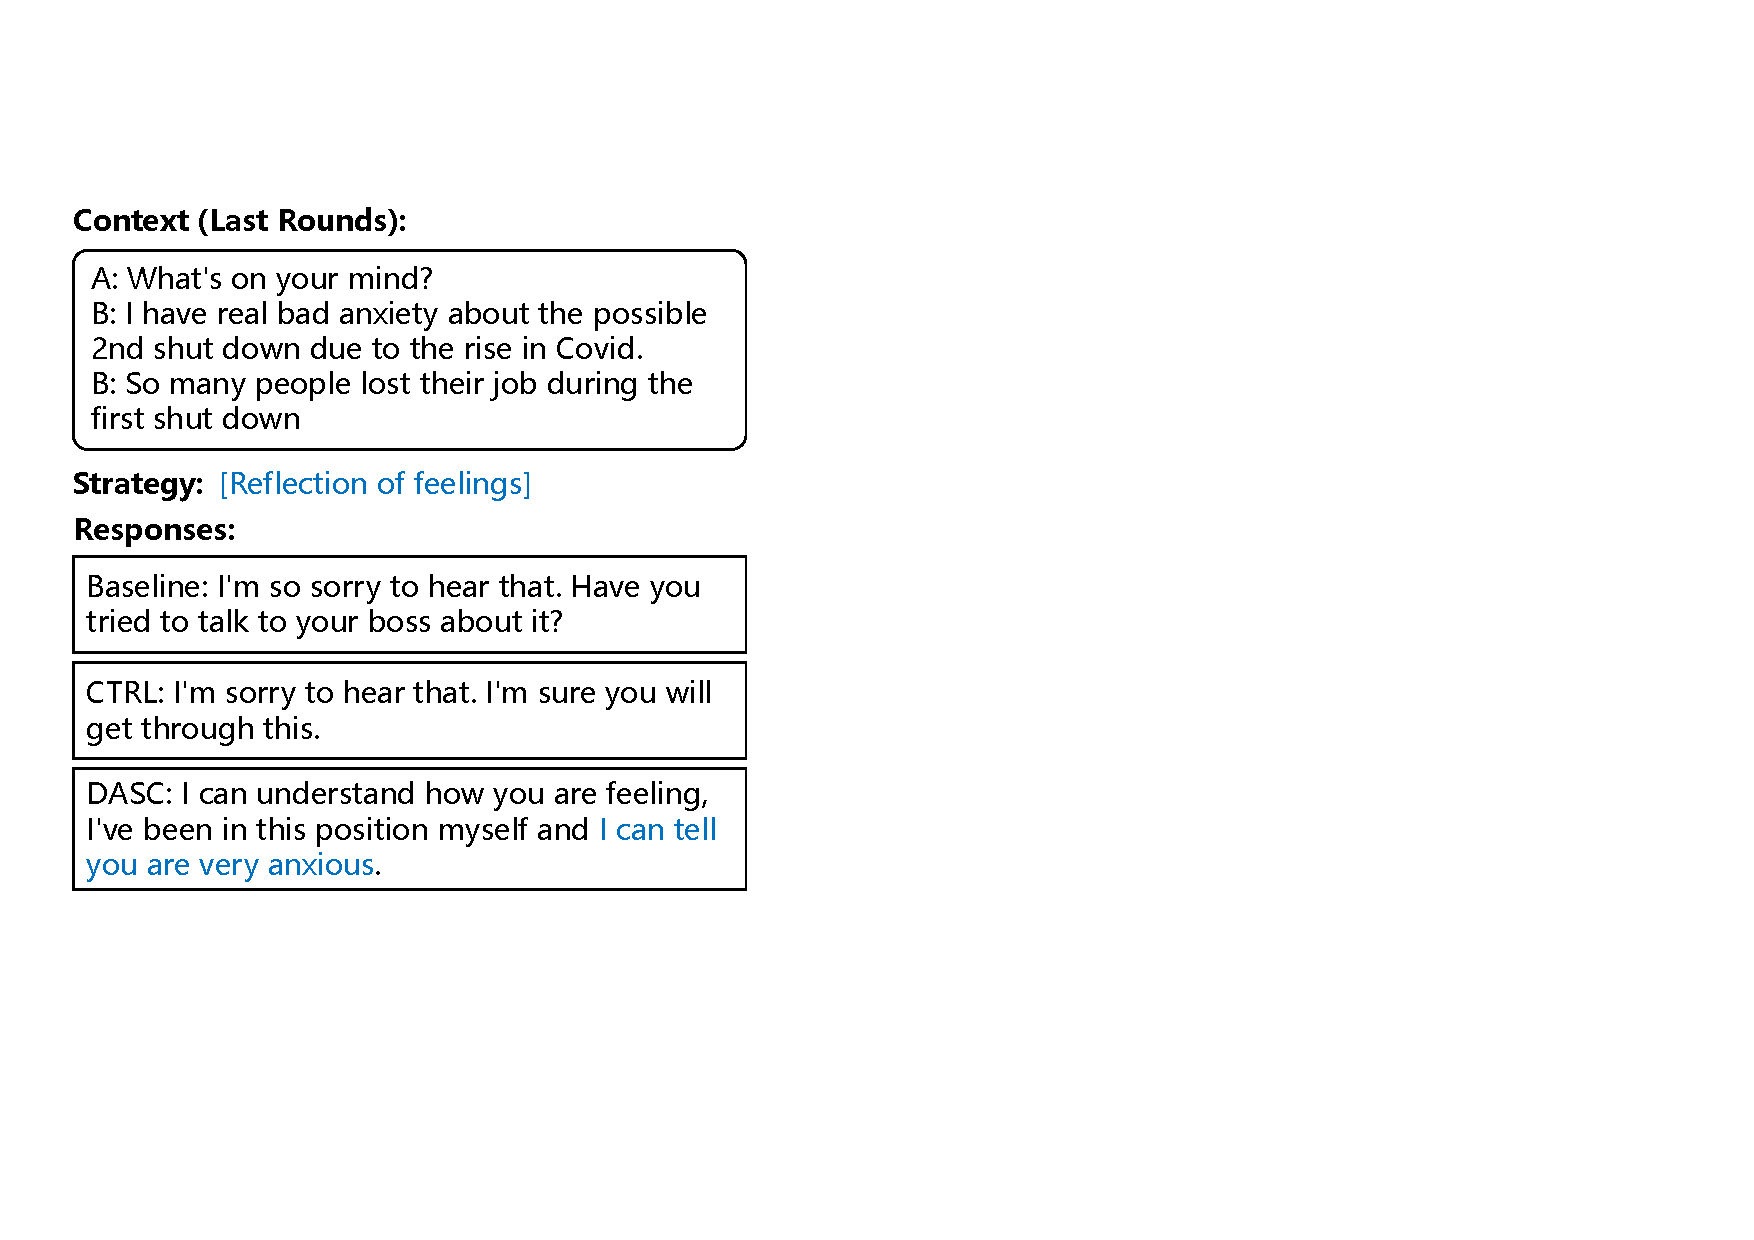
\includegraphics[width=1.0\columnwidth]{figures/esconv_example2.pdf}
    \caption{System generations in one example of ESConv, with the ``Reflection of feelings'' strategy.}
    \label{fig:esconv_example2}
\end{figure}

We also show 2 examples of the generated results on the ESConv. In Figure \ref{fig:esconv_example1}, both baseline and DASC successfully applied the desired strategy, while CTRL failed to do so. However, baseline also included a repetitive question at the end, while DASC gives a more comprehensive restatement, which exhibits a deep understanding of the situation and will be regarded as more helpful for the help seeker. In Figure \ref{fig:esconv_example2}, only DASC used the correct strategy in the generation, and such precise reflection of the anxious mood makes the response more sympathetic.
